\documentclass[a4paper,12pt]{article}
\usepackage[utf8]{inputenc}
\usepackage[MeX]{polski}
\usepackage{fixltx2e}
\usepackage[table,xcdraw]{xcolor}
\usepackage[utf8]{inputenc}
\usepackage[T1]{fontenc}
\usepackage{graphicx}
\usepackage{color}
\usepackage{mathtools}
%%%%%%%%%%%%%%%%%%%%%%%%%%%%%%%%%%%%%%%%%%%%%%%%%%%%%%%%%%%%%STRONA TYTULOWA%%%%%%%%%%%%%%%%%%%%%%%%%%%%%%%%%%%%%%%%%%%%%%%%%%%%%%%%%%%%%%%%%%%%%%%%
\title{\Huge \textbf{Politechnika Wrocławska\\[0.3in]} 
  \huge Katedra Teorii Pola, Układów elektronicznych i Optoelektronicznych \\[0.2in]
  \LARGE Zespół Układów Elektronicznych
}
\date{}
\author{}

\begin{document}
\maketitle

\begin{table}[h]
  \large
  \centering
  \begin{tabular}{|ll|l|}
    \hline
    \multicolumn{1}{|l|}{Data: 14.04.2015r}                  & \multicolumn{2}{l|}{Dzień: Wtorek}                                     \\ \hline
    \multicolumn{1}{|l|}{Grupa: VII}                        & \multicolumn{2}{l|}{Godzina: 12:15-15:00}                               \\ \hline
    \multicolumn{3}{|l|}{\textit{\begin{tabular}[c]{@{}l@{}}\textbf{Temat ćwiczenia:} \\ Przetwornice DC/DC\end{tabular}}} \\ \hline
    \textbf{Dane projektowe:}                               & \multicolumn{2}{l|}{}                                              \\
    \multicolumn{3}{|l|}{    U\textsubscript{we}=9.00 V     \quad \quad U\textsubscript{wy}=6V \quad \quad I\textsubscript{max}=0.25 A}                  \\ \hline
    \multicolumn{1}{|l|}{\textbf{l.p}}                    & \textbf{Nazwisko i imię}                 & \textbf{Oceny}               \\ \hline
    \multicolumn{1}{|l|}{1}                               & Arkadiusz Ziółkowski                     &                               \\ \hline
    \multicolumn{1}{|l|}{2}                               & Jakub Koban                              &                                \\ \hline
  \end{tabular}
\end{table}


%%%%%%%%%%%%%%%%%%%%%%%%%%%%%%%%%%%%%%%%%%%%%%%%%%%%%%%%%%%%%%%%%%%%%%%%%%%%%%%%%%%%%%%%%%%%%%%%%%%%%%%%%%%%%%%%%%%%%%%%%%%%%%%%%%%%%%%%%%%%%%%%%%%%
%%%%%%%%%%%%%%%%%%%%%%%%%%%%%%%%%%%%%%%%%%%%%%%%%%%%%%%%%%%%%%%%%%%ZADANIE PROJEKTOWE%%%%%%%%%%%%%%%%%%%%%%%%%%%%%%%%%%%%%%%%%%%%%%%%%%%%%%%%%%%%%%%
%%%%%%%%%%%%%%%%%%%%%%%%%%%%%%%%%%%%%%%%%%%%%%%%%%%%%%%%%%%%%%%%%%%%%%%%%%%%%%%%%%%%%%%%%%%%%%%%%%%%%%%%%%%%%%%%%%%%%%%%%%%%%%%%%%%%%%%%%%%%%%%%%%%%
\pagebreak
\section{Zadanie projektowe}
Zaprojektować zasilacz stabilizowany o zadanych parametrach :
\begin{itemize}
\item U\textsubscript{we}=9.00 V
\item U\textsubscript{wy}=6.00 V
\item I\textsubscript{max}=0.25 A
\end{itemize}
%%%%%%%%%%%%%%%%%%%%%%%%%%%%%%%%%%%%%%%%%%%%%%%%%%%%%%%%%%%%%%%%%%%%%%%%%%%%%%%%%%%%%%%%%%%%%%%%%%%%%%%%%%%%%%%%%%%%%%%%%%%%%%%%%%%%%%%%%%%%%%%%%%%%
%%%%%%%%%%%%%%%%%%%%%%%%%%%%%%%%%%%%%%%%%%%%%%%%%%%%%%%%%%%%%%%%%%%CZĘŚĆ PROJEKTOWA%%%%%%%%%%%%%%%%%%%%%%%%%%%%%%%%%%%%%%%%%%%%%%%%%%%%%%%%%%%%%%%%%
%%%%%%%%%%%%%%%%%%%%%%%%%%%%%%%%%%%%%%%%%%%%%%%%%%%%%%%%%%%%%%%%%%%%%%%%%%%%%%%%%%%%%%%%%%%%%%%%%%%%%%%%%%%%%%%%%%%%%%%%%%%%%%%%%%%%%%%%%%%%%%%%%%%%
\section{Obliczenia projektowe}

\begin{equation}
I_{pk}=I_{Lpk}=2I_{0max}=2*0.25=0.5 A
\end{equation}

\begin{equation}
\mathbf{R_{SC}}=\frac{0.3V}{I_{pk}}=\frac{0.3}{0.5}=\mathbf{0.6 \Omega}
\end{equation}

\begin{equation}
Zakładamy \quad \mathbf{R_1=1.8k\Omega}   \quad \to \quad   \mathbf{R_2}=R_1 \frac {|U_0|-1.25V}{1.25V} = 1800\frac{6-1.25}{1.25}= \mathbf{6.8k \Omega}
\end{equation}

\begin{equation}
Zakładamy \quad \mathbf{T=25u}s \quad \to \quad \mathbf{t_{on}}=T\frac{U_0}{U_i}=25*10^{-6}\frac{6}{9}=\mathbf{16.67us}
\end{equation}

\begin{equation}
\mathbf{L}\geq\frac{U_i}{I_{Lpk}}t_{ON}=\frac{9}{0.5}*16.37*10^{-6}=\mathbf{300uH}
\end{equation}

\begin{equation}
\mathbf{C_0}\geq\frac{I_{Lpk}T}{8U_{tpp}}=\frac{0.5*25*10^{-6}}{8*0.5}=\mathbf{3.125uF}
\end{equation}

%%%%%%%%%%%%%%%%%%%%%%%%%%%%%%%%%%%%%%%%%%%%%%%%%%%%%%%%%%%%%%%%%%%%%%%%%%%%%%%%%%%%%%%%%%%%%%%%%%%%%%%%%%%%%%%%%%%%%%%%%%%%%%%%%%%%%%%%%%%%%%%%%%%%
\section {Schemat projektowy}
\begin{figure}[h]
  \center
  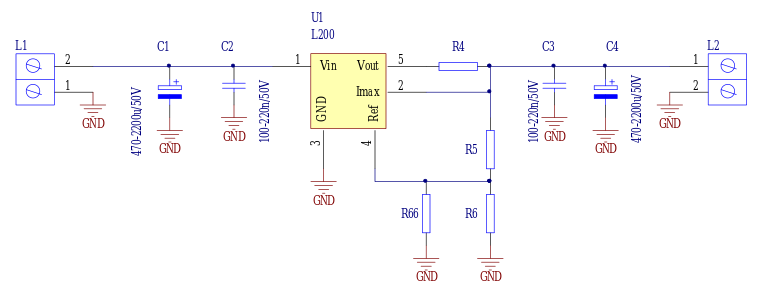
\includegraphics[width=1\textwidth]{schemat_ukladu}
  \caption{Schemat projektowanego układu}
\end{figure}
\pagebreak
%%%%%%%%%%%%%%%%%%%%%%%%%%%%%%%%%%%%%%%%%%%%%%%%%%%%%%%%%%%%%%%%%%%%%%%%%%%%%%%%%%%%%%%%%%%%%%%%%%%%%%%%%%%%%%%%%%%%%%%%%%%%%%%%%%%%%%%%%%%%%%%%%%%%
%%%%%%%%%%%%%%%%%%%%%%%%%%%%%%%%%%%%%%%%%%%%%%%%%%%%%%%%%%%%%%%%%%%CZĘŚĆ LABORATORYJNA%%%%%%%%%%%%%%%%%%%%%%%%%%%%%%%%%%%%%%%%%%%%%%%%%%%%%%%%%%%%%%
%%%%%%%%%%%%%%%%%%%%%%%%%%%%%%%%%%%%%%%%%%%%%%%%%%%%%%%%%%%%%%%%%%%%%%%%%%%%%%%%%%%%%%%%%%%%%%%%%%%%%%%%%%%%%%%%%%%%%%%%%%%%%%%%%%%%%%%%%%%%%%%%%%%%
\section{Część laboratoryjna}
\subsection{Charakterystyki napięciowe}
TUTAJ BRAKUJE 2 tabeli ale nie wiem czy mogę tak bezczelnie uwalić część danych :p >>DO SKONSULTOWANIA<<
\begin{table}[ht]
  \centering
  \begin{tabular}{|r|r|}
    \hline
    \multicolumn{1}{|c|}{\textbf{U1{[}V{]}}} & \multicolumn{1}{c|}{\textbf{U2\_1 {[}V{]}}} \\ \hline
    0                                        & 0                                           \\ \hline
    2                                        & 0.2862                                      \\ \hline
    5                                        & 4.0874                                      \\ \hline
    5.5                                      & 4.561                                       \\ \hline
    8                                        & 6.988                                       \\ \hline
    8.5                                      & 7.457                                       \\ \hline
    9                                        & 7.874                                       \\ \hline
    10.1                                     & 8.916                                       \\ \hline
    10.5                                     & 9.32                                        \\ \hline
    11                                       & 9.87                                        \\ \hline
    11.5                                     & 10.35                                       \\ \hline
    12                                       & 10.784                                      \\ \hline
    12.5                                     & 10.992                                      \\ \hline
    13                                       & 10.994                                      \\ \hline
    13.5                                     & 10.994                                      \\ \hline
    14                                       & 10.995                                      \\ \hline
    14.5                                     & 10.995                                      \\ \hline
    15                                       & 10.995                                      \\ \hline
    17                                       & 10.999                                      \\ \hline
    19                                       & 11                                          \\ \hline
    20                                       & 11.002                                      \\ \hline
    25                                       & 11.007                                      \\ \hline
    30                                       & 11.014                                      \\ \hline
  \end{tabular}
\end{table}
\pagebreak
%%%%%%%%%%%%%%%%%%%%%%%%%%%%%%%%%%%%%%%%%%%%%%%%%%%%%%%%%%%%%%%%%%%%%%%%%%%%%%%%%%%%%%%%%%%%%%%%%%%%%%%%%%%%%%%%%%%%%%%%%%%%%%%%%%%%%%%%%%%%%%%%%%%%

\begin{figure}[h!]
  \center
  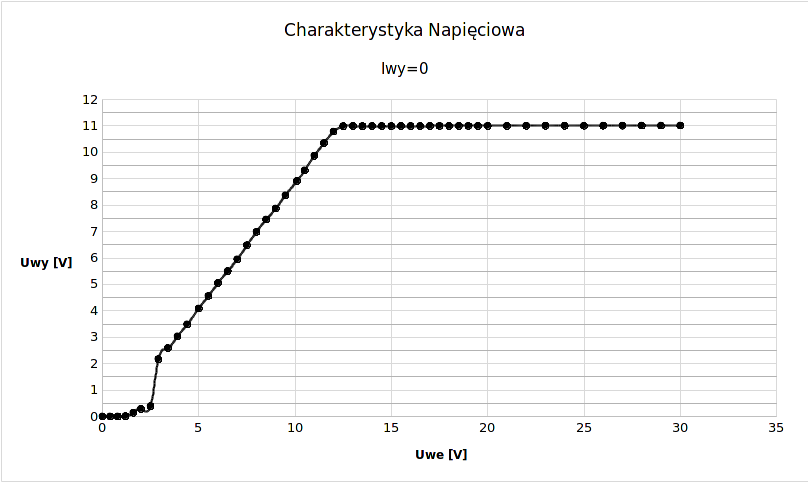
\includegraphics[width=0.90\textwidth]{charak-napieciowa1}
  \caption{U\textsubscript{wy}=f(I\textsubscript{wy}) przu I\textsubscript{wy}=0A}
\end{figure}

\begin{figure}[h!]
  \center
  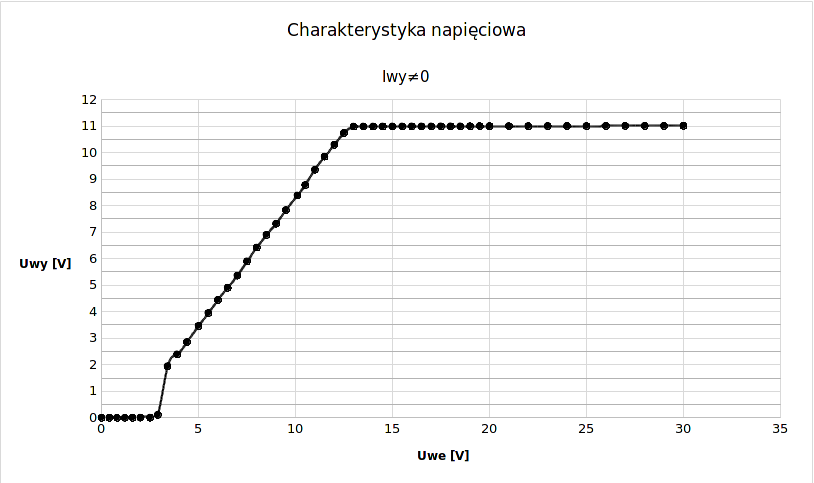
\includegraphics[width=0.90\textwidth]{charak-napieciowa2}
  \caption{U\textsubscript{wy}=f(U\textsubscript{we}) przu I\textsubscript{wy}\neq0A}
\end{figure}

Analizując przedstawione charakterystyki możemy zauważyć,iż układ poprawnie stabilizuje napięcie od (odpowiednio) 12.5V i 13V aż do maksymalnego
napięcia jakie udało nam się uzyskać z zasilacza czyli 30V.
\pagebreak
%%%%%%%%%%%%%%%%%%%%%%%%%%%%%%%%%%%%%%%%%%%%%%%%%%%%%%%%%%%%%%%%%%%%%%%%%%%%%%%%%%%%%%%%%%%%%%%%%%%%%%%%%%%%%%%%%%%%%%%%%%%%%%%%%%%%%%%%%%%%%%%%%%%%
\subsection{Charakterystyki zewnętrzne}

\begin{figure}[h]
  \center
  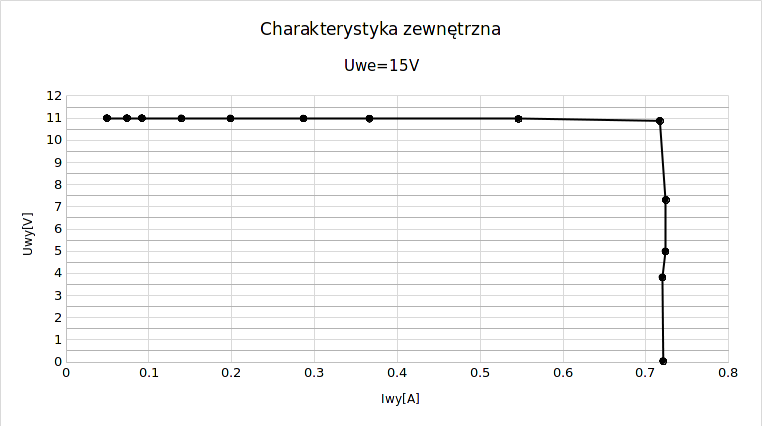
\includegraphics[width=0.75\textwidth]{charak-zew1}
  \caption{U\textsubscript{wy}=f(I\textsubscript{wy}) przu U\textsubscript{we}=15V}
\end{figure}

\begin{figure}[h]
  \center
  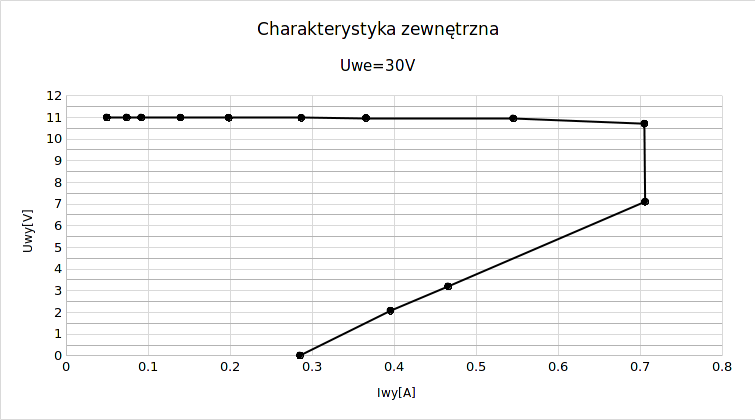
\includegraphics[width=0.75\textwidth]{charak-zew2}
  \caption{U\textsubscript{wy}=f(I\textsubscript{wy}) przu U\textsubscript{we}=30V}
\end{figure}

Analizując charakterystyki zewnętrzne stabilizatora zauważamy, że przy U\textsubscript{we}=15V układ nie przepuszcza prądu powyżej zadanych 0.70A,
natomiast przy U\textsubscript{we}=30V obserwujemy tzw. foldback ('odwijanie' charakterystyki) co jest zabezpieczeniem układu w wypadku dalszego
wzrostu napięcia wejściowego.
%%%%%%%%%%%%%%%%%%%%%%%%%%%%%%%%%%%%%%%%%%%%%%%%%%%%%%%%%%%%%%%%%%%%%%%%%%%%%%%%%%%%%%%%%%%%%%%%%%%%%%%%%%%%%%%%%%%%%%%%%%%%%%%%%%%%%%%%%%%%%%%%%%%%

\section {Wnioski}

\begin{enumerate}  
\item Zgodnie z założeniami teoretycznymi układ utrzymuje na swoim wyjściu stałe napięcie równe 11V , w związku z niedokładnością użytych
  elementów maksymalny prąd wyjściowy różni się od założeń jednak nie jest to duża rozbieżność (około 0.70 A wobec założonych 0.60 A).
\item Minimalne napięcie dla jakiego układ pracuje poprawnie przy I\textsubscript{wy}=0 to 12.5V a dla I\textsubscript{wy}\neq0$ to 13V.
\item W stabilizatorze kompensacyjnym użyto tzw. foldback'u który jest bardzo dobrym zabezpieczeniem układu w wypadku podawania na wejście zbyt
  dużych wartości napięć.
\end{enumerate}



\end{document}
